\documentclass[25pt, a0paper, landscape, cmyk]{tikzposter}
\usepackage{hyperref}
\tikzposterlatexaffectionproofoff
\title{Edit Conflicts, Offline Contributions, and Tor: Oh, My!}
\author{C. Scott Ananian / cananian@wikimedia.org / \texttt{[[User:cscott]]}}
\institute{Wikimedia Foundation}
%\usetheme{Autumn}\usecolorstyle[colorPalette=BrownBlueOrange]{Britain}
%\usetheme{Envelope}
\usetheme{Rays}\usecolorstyle[colorOne=orange,colorTwo=green]{Australia}

% Work around tikzposter conflict with hyperref
% https://tex.stackexchange.com/questions/254257/tikzposter-and-doi-package-conflict
\def\HyperFirstAtBeginDocument#1{#1}

\begin{document}\maketitle[width=75cm]%[titletextscale=1,width=75cm]
\begin{columns}
  \column{0.33}
  \block{Editing Conflicts}{%

    \begin{tikzfigure}
      
\includegraphics[height=12.5cm]{conflict-silhouette.eps}
    \end{tikzfigure}

    A new editor makes a contribution. It is immediately reverted and
    their work is apparently "lost".

    \begin{quote}
    A careful editor wants a space to refine and get feedback on a
    draft edit over a period of time, without worrying about unrelated
    edits causing conflicts.
    \end{quote}

    A user encounters an edit conflict and gives up.

    \begin{quote}
    A computer crash just before publishing a long edit causes all
    work to be lost.
    \end{quote}

    A minority editor wants a safe space to work without
    immediate harassment.
  }
  \column{0.34}
  \block{Offline Contributions}{%

    \begin{tikzfigure}
      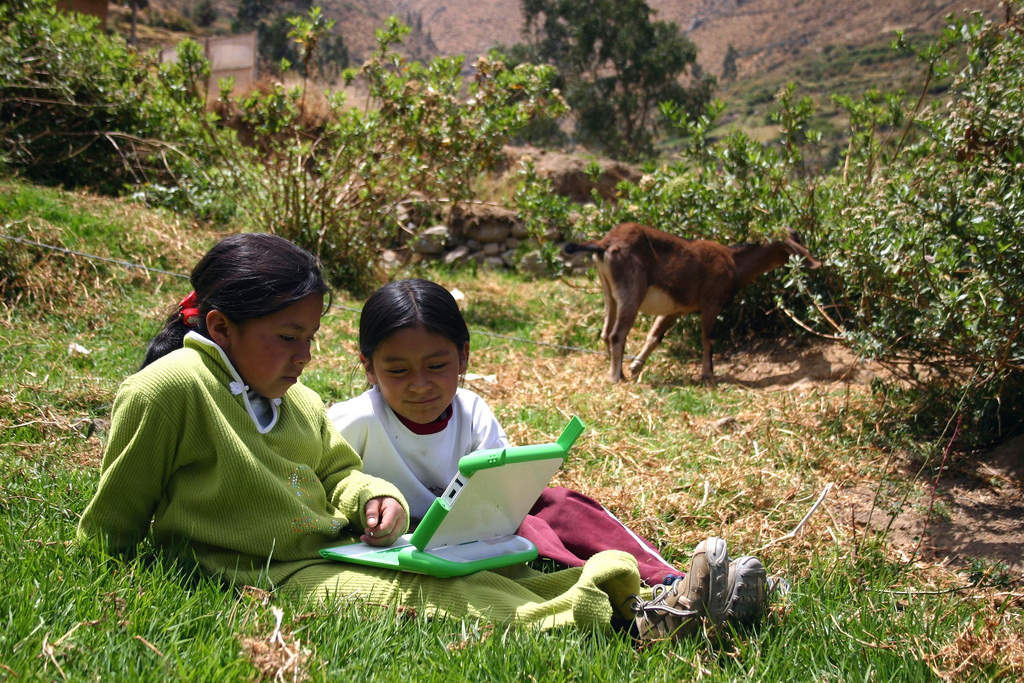
\includegraphics[height=20cm]{Bucolico-full.jpg}
    \end{tikzfigure}

    A Peruvian school-child finds no information in Wikipedia about
    their hometown, but can't contribute an article because they are
    using the wiki offline.

  }
  \column{0.33}
  \block{Tor!}{%

    \begin{tikzfigure}
      
\includegraphics[height=20cm]{censored-nospeaking.eps}
    \end{tikzfigure}

    A user in a repressive regime can only safely access Wikipedia by
    using Tor, but in a catch-22 they then lose the ability to make
    contributions.

  }
\end{columns}
\block{}{\centering\Huge\it Oh, my!}
\begin{columns}
  \column{0.33}
  \block{Fork-Merge}{%

    With a fork-and-merge model new users whose content isn't
    immediately merged find it preserved on their fork for revision
    and re-submission, reducing their sense of rejection and
    loss. Offline users who are forced to work on an out-of-date copy
    and those using the draft namespace can use the same improved
    tools when their contributions are brought to merge. During online
    edits we can auto-save to a fork, and if conflicts are found we
    can safely defer resolving them without losing work.

  }
  \column{0.34}
  \block{Collaborative Edit Queues}{%
With volunteer-run queues for merging contributions, we can incorporate contributions from offline editors or Tor users, or rescue conflicted edit attempts.

    \centering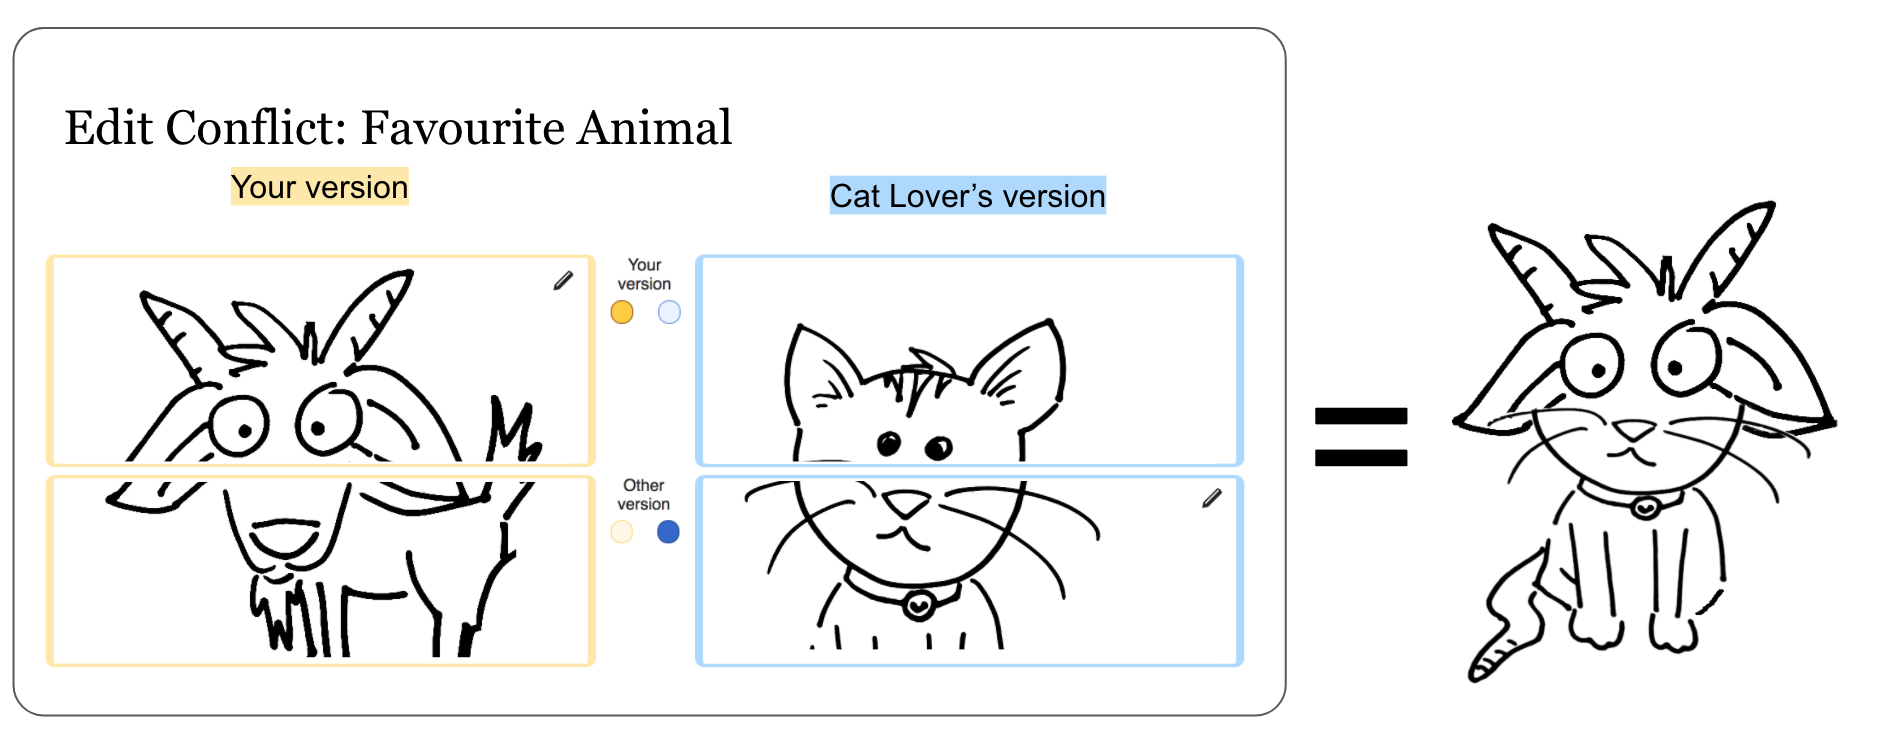
\includegraphics[height=10cm]{favourite-animal.png}
}
  \column{0.33}
  \block{Volunteer Communities}{%
  We then can collect edits from more diverse and less-connected users
and provide a friendlier first-edit experience to retain
newcomers. Volunteer merge queues provide another means for those
well-connected to aid those with difficulties in the spirit of
ubuntu. By increasing participation we can bridge the knowledge gap.

\begin{tikzfigure}
  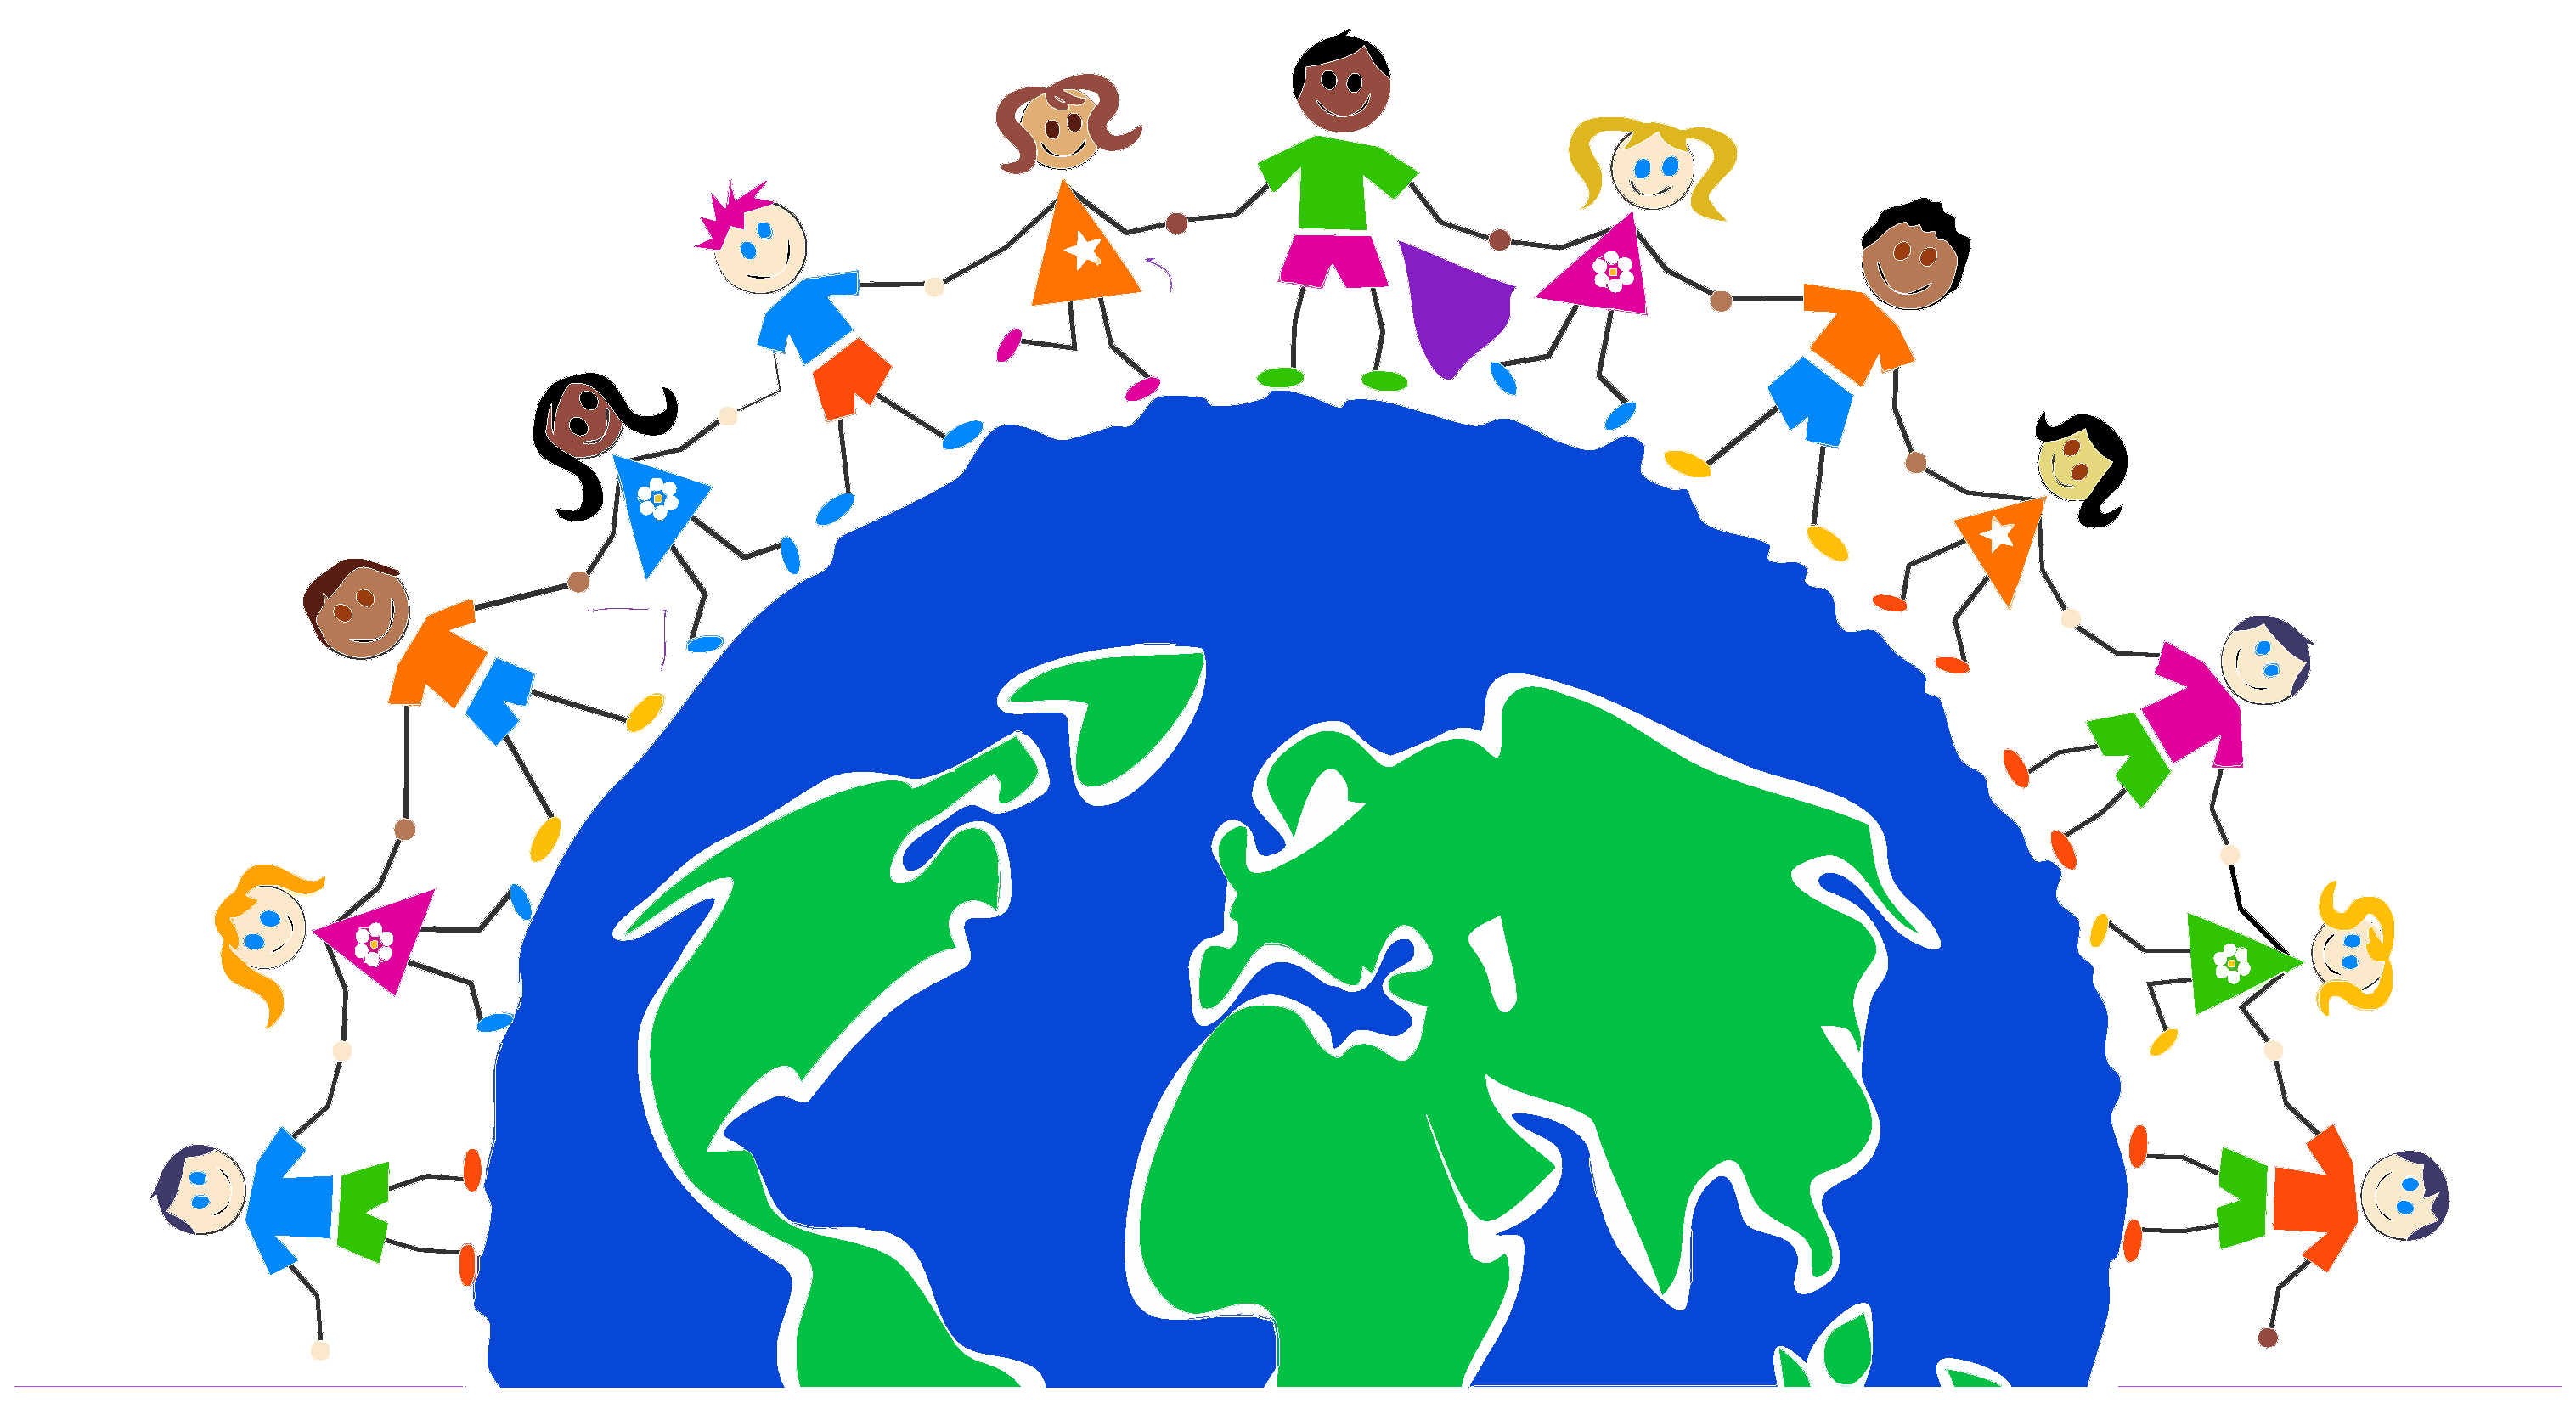
\includegraphics[height=10cm]{world-kids-nobg.eps}
\end{tikzfigure}
}
\end{columns}
\block{}{\centering\tiny
  \href{https://openclipart.org/detail/231887/conflict-silhouette}{conflict-silhouette}
    by \href{https://openclipart.org/user-detail/GDJ}{GDJ}
    / \href{http://creativecommons.org/publicdomain/zero/1.0/}{CC0};
  \url{http://wiki.laptop.org/go/File:Bucolico-full.jpg}
    by OLPC Peru
    / \href{https://creativecommons.org/licenses/by-sa/4.0/legalcode}{CC-SA};
  \href{https://openclipart.org/detail/296265/censored-no-speaking}{censored-no-speaking}
    by \href{https://openclipart.org/user-detail/j4p4n}{j4p4n}
    / \href{http://creativecommons.org/publicdomain/zero/1.0/}{CC0};
  \href{https://openclipart.org/detail/228325/world-kids}{world-kids}
    by \href{https://openclipart.org/user-detail/GDJ}{GDJ}
    / \href{http://creativecommons.org/publicdomain/zero/1.0/}{CC0}
    / Background removed;
  \href{https://commons.wikimedia.org/wiki/File:Paragraph-based_prototype_\%E2\%80\%93_rough_visualization_of_the_functionality.png}{Edit conflict}
    by \href{https://commons.wikimedia.org/wiki/User:Johanna_Strodt_(WMDE)}{Johanna\_Strodt\_(WMDE)}
    / \href{https://creativecommons.org/licenses/by-sa/4.0/legalcode}{CC-SA};
}
\end{document}
